% siminos/reversal/recip1d.tex      pdflatex LC21; bibtex LC21
% temporary:  siminos/spatiotemp/chapter/LC21recip1d.tex
% $Author: hanliang $ $Date: 2021-12-24 16:09:56 -0500 (Fri, 24 Dec 2021) $

% Predrag 2021-08-08: shared with siminos/reversal/LC21.tex

\section{Reciprocal lattice}
\label{sect:LC21recip1d} % started with {sect:RhombCornerFT}

Think of a solution of a discrete time dynamical system as a 1\dmn\
temporal {\lattstate} with the field on each site labeled by integer
time.
A period-$\cl{}$ {\lattstate} lives on a discrete 1-torus (a ring or chain or
necklace) of period-$\cl{}$, and if its law is time-invariant, its orbit, the set of
{\lattstate}s related to it by cyclic translations, are
physically equivalent. The symmetry is the cyclic group
\Cn{n}, and one only needs to count and distinguish \Cn{n} \emph{{\orbit}s},
compute only one {\lattstate} per each orbit.

The smart way to do this is by going to the irreducible representations
of \Cn{n} by discrete Fourier transform.
Were the lattice $d$\dmn, defined by Bravais cell vectors $\{\mathbf{a}\}$, a
crystallographer would immediately move to the \emph{reciprocal}
lattice,
\( %beq
\tilde{\lattice}_{\mathbf{b}} = \{k \mathbf{b}\,|\, k \in \mathbb{Z}\}
\,,
\) %ee{LC21:Rcpr1dLatt}
with {reciprocal}
lattice basis vectors $\{\mathbf{b}\}$ satisfing
\( %beq
\mathbf{b} \cdot \mathbf{a} = 2 \pi
\,.
\) %ee{LC21:Rcpr1dVect}
On the {reciprocal} lattice translations are
quotiented out, and calculations are restricted to a finite
{Brilluoin zone} (this is the {`Bloch theorem'} of
solid state physics). Here we work on a 1\dmn\ lattice with unit
lattice spacing 1, so the reciprocal lattice spacing is $2\pi/1=2\pi$, with
the (first) Brillouin zone from $k=-\pi$ to $k=\pi$.


The group elements of the \Cn{n} permutation representation
are generated by
the $[\cl{}\!\times\!\cl{}]$ shift matrix
\refeq{hopMatrix} which
 translates for\-ward-in-time a {\lattstate} \refeq{1dLattStatC_n} by one site,
$\transp{(\shift \Xx)}=(\ssp_1,\ssp_2,\cdots,\ssp_{\cl{}-1},\ssp_0)$.
After $\cl{}$ shifts, the {\lattstate} returns to the initial
state, yielding the characteristic equation for the matrix $\shift$
\beq
\shift^\cl{}-\id=0
\,,
\ee{shift2n}
whose eigenvalues are $\cl{}$th roots of unity, with the $\cl{}$ complex
eigenvectors also built from roots of unity
\bea
\{\lambda_k\} &=& \{1, \omega, \omega^2,\cdots, \omega^{\cl{}-1}\}
                \,,\qquad\qquad\quad
                  \omega=\e^{2\pi\mathrm{i}/\cl{}}
                \continue
\tilde{e}_k   &=&
    \frac{1}{\sqrt{\cl{}}}
    (1, \omega^k, \omega^{2k}, \ldots, \omega^{k(\cl{}-1)})
    \,,\qquad k=0, 1,\ldots, \cl{}-1
\,.
\label{FourierModes}
\eea
In the $\{\tilde{e}_k\}$ discrete Fourier basis, a real $\cl{}$\dmn\
{\lattstate} vector $\Xx$ is mapped onto a $\cl{}$\dmn\ complex
{reciprocal} lattice  vector
\beq
\tilde{\Xx} = (\cssp_{0},\cssp_{1},\cssp_{2},\dots,\cssp_{\cl{}-1})
\,.
\eeq
The $k$th Fourier mode has magnitude $|\cssp_k|$ and phase $e^{i\theta_k}$.

On the reciprocal lattice, the dynamics is breathtakingly simple: no
matter what the dynamical system is, all reciprocal {\lattstate}s
literally run in circles.
The shift matrix is diagonal, $\shift_{jk}=\omega^k\,\delta_{jk}$,
and when the shift operator acts on the {\lattstate}, $\Xx \to \shift \Xx$,
the $k$th Fourier mode magnitude $|\cssp_k|$ remains the same, while
its phase is incremented by an $\cl{}$th fraction of the circle:
\bea
(\ssp_0,\ssp_1,\ssp_2,\cdots,\ssp_{\cl{}-1}) &\to&
    (\ssp_1,\ssp_2,\cdots,\ssp_{\cl{}-1},\ssp_0)
\continue
e^{\mathrm{i}\theta_k} &\to& \omega^k e^{i\theta_k}
                      = e^{\mathrm{i}(\theta_k+2\pi{k}/\cl{})}
\,.
\eea
In other words, for non-zero $k$ and $|\cssp_k|$, all reciprocal
{\lattstate}s lie in complex plane on vertices of regular $\cl{}$-gons,
inscribed in circles of radius $|\cssp_k|$, one for each orbit.

As a concrete example, consider first the 7 period-3 {\lattstate}s of
the temporal Bernoulli \refeq{1stepDiffEq} for stretching parameter $s=2$.
It is a linear problem and all {\lattstate}s are easily computed
by hand, one for each $\Mm$. There is always the 3rd repeat of the
fixed point {\lattstate} $(0,0,0)$, and the remining 6 {\lattstate}s
belong to 2 period-3 orbits, which we mark by a single {\lattstate}
per orbit, for example
$(\frac{1}{7},\frac{2}{7},\frac{4}{7})$
and
$(\frac{3}{7},\frac{6}{7},\frac{5}{7})$.
Discrete Fourier transform maps
these 7 {\lattstate}s into 7 reciprocal {\lattstate}s of \reffig{fig:BernC3}.

Consider next the action of the shift operator $\shift$ on the reciprocal
{\lattstate}s. The $k=0$ component of any reciprocal {\lattstate} is
invariant under the shift. In the $k=1$ and $k=2$ subspaces, the shift
$\shift$ acts by complex phase rotations $\exp(2 \pi \mathrm{i}/3)$ and
$\exp(4 \pi \mathrm{i}/3)$, respectively: reciprocal {\lattstate}s that
belong to the same orbit lie on a circle in the complex plane, and are
related by complex rotations. \refFig{fig:BernC3} illustrates
this; the two period-3 orbits, built from reciprocal {\lattstate}s that
are related by shifts, are connected by blue lines.


%%%%%%%%%%%%%%%%%%%%%%%%%%%%%%%%%%%%%%%%%%%%%%%%%%%
\begin{figure}
  \centering
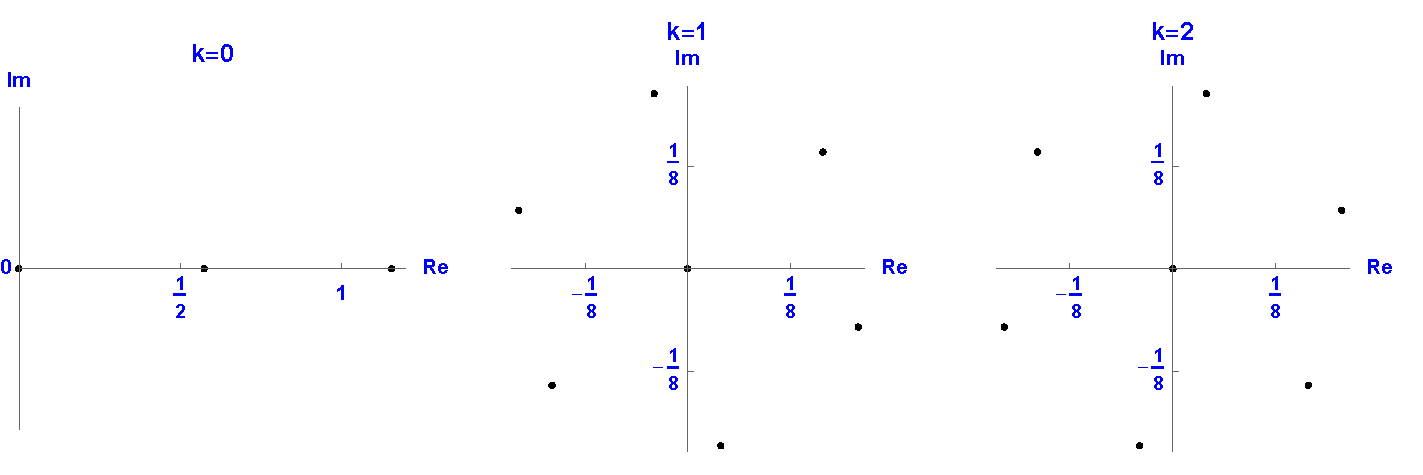
\includegraphics[width=\textwidth]{HLBernoulliC3}
  \caption{\label{fig:BernC3}
The three reciprocal lattice $(\cssp_{0},\cssp_{1},\cssp_{2})$ Fourier
components representation of the 7 $\Cn{3}$-equivariant period-3
{\lattstate}s, $s=2$ {temporal Bernoulli system} \refeq{1stepDiffEq}. In
$\cssp_1$ and $\cssp_2$ complex planes, reciprocal {\lattstate}s lie on
vertices of the 2 equilateral triangles. They comprise the 2 distinct
\Cn{3} orbits, while the state at the origin is the fixed point
$\Xx=(0,0,0)$.
}
\end{figure}
%%%%%%%%%%%%%%%%%%%%%%%%%%%%%%%%%%%%%%%%%%%%%%%%%%%

%%%%%%%%%%%%%%%%%%%%%%%%%%%%%%%%%%%%%%%%%%%%%%%%%%%%%%%%%%%%%%%%%%%%%
% 2021-01-27 Han: figSrc/han/Mathematica/HLFourier5cycles.nb
%                                    HLFourierTranform5Cycles.nb
\begin{figure}
  \centering
{(a)} %$\!\!\!\!$
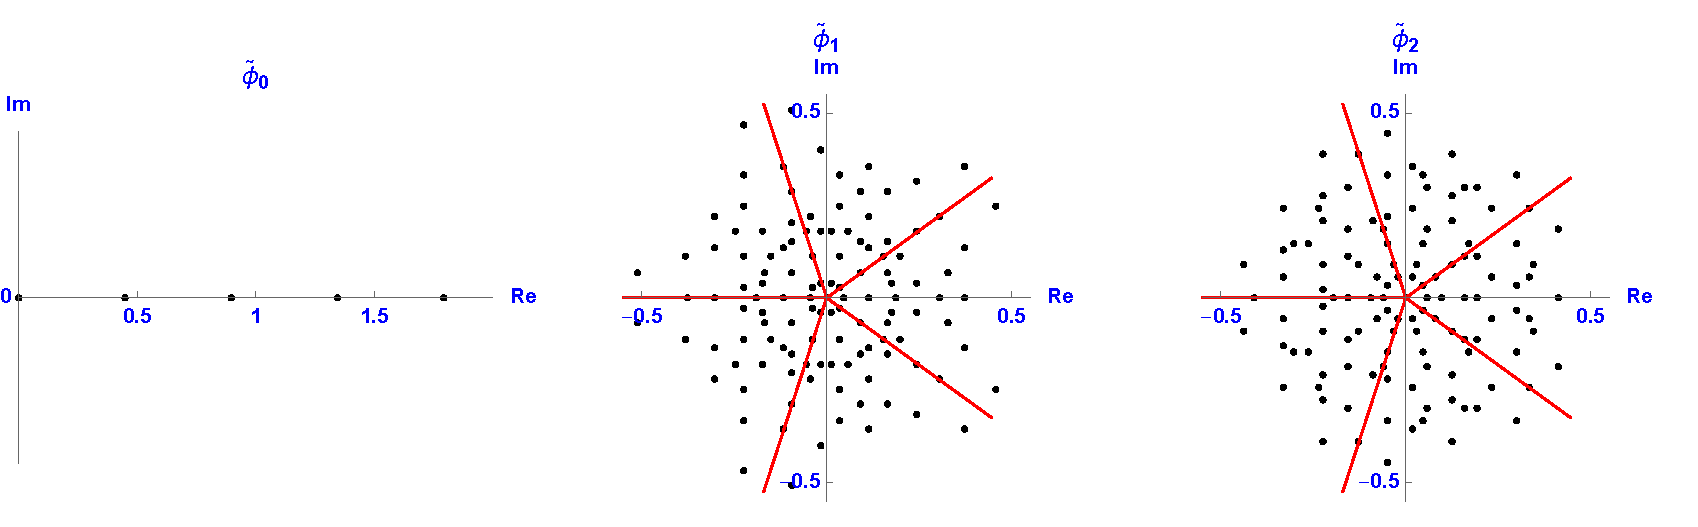
\includegraphics[width=0.9\textwidth]{HLFourierFieldLength5}
~~~
\\
{(b)} %$\!\!\!\!$
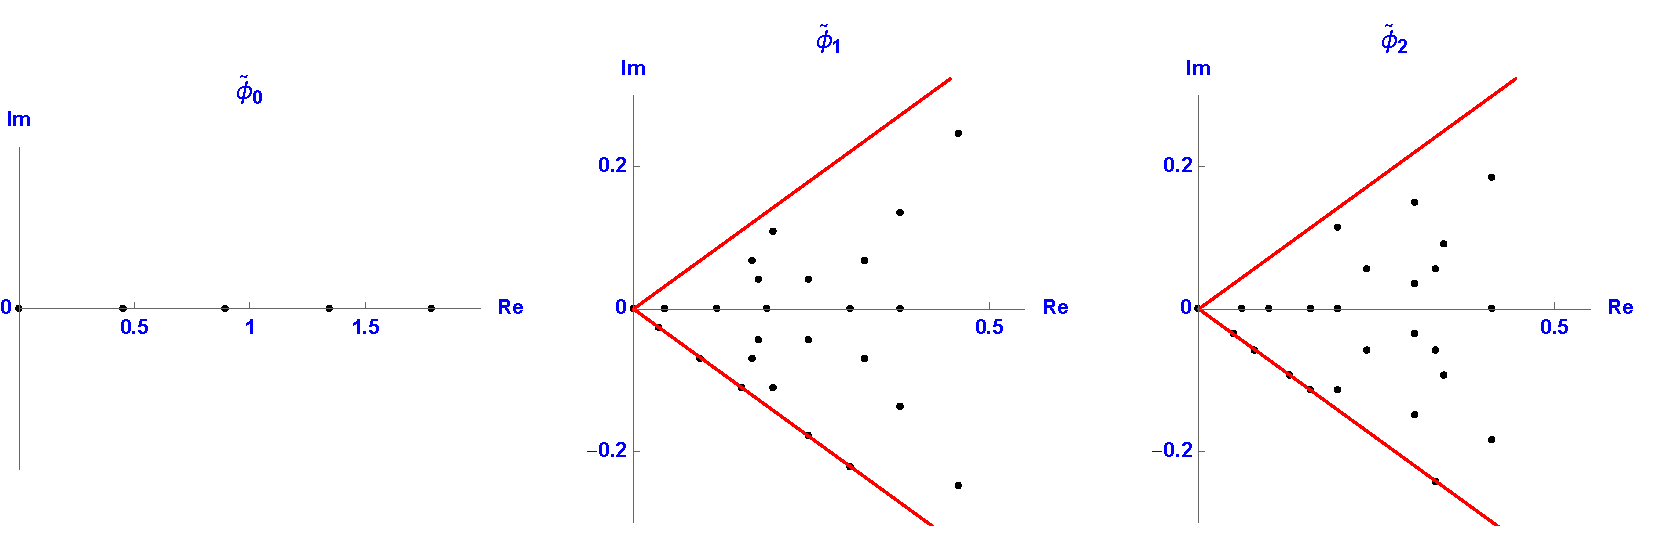
\includegraphics[width=0.9\textwidth]{HLFundFieldLength5}
\\ %~~~
  \caption{\label{fig:templattC5} % in blog {fig:HLFundFieldLength5}
The 121 period-5 reciprocal {\lattstate}s
of the $s=3$ \templatt\ \refeq{catMapNewt}.
    (a)
The $k=0,1,2$ Fourier component complex planes (by \templatt\ time
reversal invariance, $k=3$ has the same orbits as $k=2$, and  $k=4$ as
$k=1$).
The state at the origin is the fixed point $(0,0,0,0,0)$.
As in \reffig{fig:BernC3}, all non-zero reciprocal {\lattstate}s
lie on vertices of pentagons that form orbits under \Cn{5} cyclic permutations.
    (b)
A \Cn{5} fundamental domain contains non-zero  reciprocal
{\lattstate}s whose phases lie in the $[-2\pi/10,2\pi/10)$ wedge, one reciprocal
{\lattstate} for each distinct \Cn{5} orbit.
          }
\end{figure}
%%%%%%%%%%%%%%%%%%%%%%%%%%%%%%%%%%%%%%%%%%%%%%%%%%%%%%%%%%%%%%


\subsection{Fundamental domain} % of the {\lattstate}}

As a next example, consider the 121 period-5 reciprocal {\lattstate}s
of the $s=3$ \templatt\ \refeq{catMapNewt} plotted in \reffig{fig:templattC5}.
The number of {\lattstate}s in the fundamental domain is 25. One of
them is the constant $\{0,0,0,0,0\}$ state. Each one of the other, prime
solutions contributes 5 times to $N_5$, the total number of {\lattstate}s
belong to the same time orbit. So we have the total number of solutions:
$N_5=121=1+M_5\times5 = 1+24\times5$, see  \reftab{tab:catMapN_n-s=3}.


repeats of shorter {\lattstate}s sit on the boundaries of the fundamental domain.
Lattice shift $\shift_j$ maps out the $\Group$-orbit by running on
circles, and orbits visit the $1/2\cl{}$ wedge only once, so the points
in the fundamental domain represent an orbit each.


Given the space of the field configuration and the symmetry group acting on it,
we can find a fundamental domain such that each orbit in this space
visits the fundamental domain only once.
Each {\lattstate} in the fundamental domain is a representative {\lattstate} of an
orbit.
    \PC{2021-10-12}{
    Please read our draft\rf{LC21}, and either follow
    our definition \refeq{1dLattStat} of {\em {\lattstate}},
    or replace it with some other definition.
    }

One method to find the fundamental domain is based on the decomposition
of the space into the subspaces of the irreps of the symmetry group.
A natural way to choose the fundamental domain is to divide in the
subspace of an irrep, where the irrep divides the subspace into the number
of copies that is equal to the order of the symmetry group.

For example, in the space of the field configuration with \Cn{\cl{}} symmetry, the $k=1$ subspace
spanned by the eigenstate $\tilde{e}_1$, defined in \refeq{FourierModes}, can be divided
into $\cl{}$ copies. One can choose the region in the complex plane of $k=1$ subspace
with argument $\pi/\cl{}\leq\arg(\cssp_{1})<\pi/\cl{}$ to be the fundamental domain.
Each orbit can visit the fundamental domain only once. As shown in \reffig{fig:BernC3},
there are 3 points in this region, which are representative {\lattstate}s of two different
period-3 orbits and the fixed point $0$.
